%\documentclass[tikz, border=5pt]{standalone}
\begin{document}
	% 图(1)
	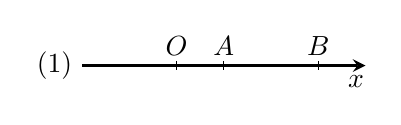
\begin{tikzpicture}[scale=0.6]
		\node[left] at (-1, 0) {(1)};            % 左编号
		% 绘制主水平线
		\draw[->, >=stealth, line width=1pt] (-1,0) -- (5,0);
		\node[below] at (4.8,0) {$x$};
	
		% 6个小竖线标记点(从左到右)
		\draw (1,0.1) -- (1,-0.1); \node[above] at (1,0) {$O$};   % 第一个竖线标记
		\draw (2,0.1) -- (2,-0.1); \node[above] at (2,0) {$A$};   % 第二个竖线标记
		\draw (4,0.1) -- (4,-0.1); \node[above] at (4,0) {$B$};   % 第三个竖线标记
	\end{tikzpicture}
	
	% 图(2)
	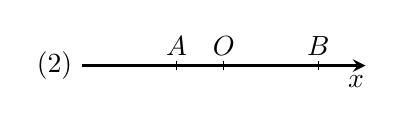
\begin{tikzpicture}[scale=0.6]
		\node[left] at (-1, 0) {(2)}; 		% 左编号
		\draw[->, >=stealth, line width=1pt] (-1,0) -- (5,0); 		% 绘制水平线
		\node[below] at (4.8,0) {$x$}; 
		\foreach \pos/\label in {1/A, 2/O, 4/B} {    % 点O、A、B的位置
			\draw (\pos, 0.1) -- (\pos, -0.1);       % 竖线标记
			\node[above] at (\pos, 0) {$\label$};    % 点标签(上方)
		}
	\end{tikzpicture}
	
	% 图(3)
	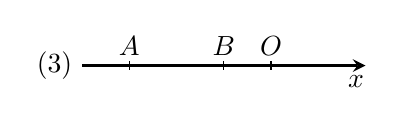
\begin{tikzpicture}[scale=0.6]
		\node[left] at (-1, 0) {(3)}; 		% 左编号
		\draw[->, >=stealth, line width=1pt] (-1,0) -- (5,0); 		% 绘制水平线
		\node[below] at (4.8,0) {$x$}; 
		\foreach \pos/\label in {0/A, 2/B, 3/O} {
			\draw (\pos, 0.1) -- (\pos, -0.1);
			\node[above] at (\pos, 0) {$\label$};
		}
	\end{tikzpicture}
	
	% 图(4)
	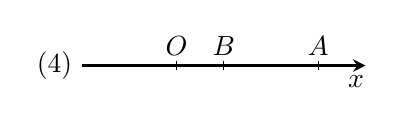
\begin{tikzpicture}[scale=0.6]
		\node[left] at (-1, 0) {(4)}; 		% 左编号
		\draw[->, >=stealth, line width=1pt] (-1,0) -- (5,0); 		% 绘制水平线
		\node[below] at (4.8,0) {$x$}; 
		\foreach \pos/\label in {1/O, 2/B, 4/A} {
			\draw (\pos, 0.1) -- (\pos, -0.1);
			\node[above] at (\pos, 0) {$\label$};
		}
	\end{tikzpicture}
	
	% 图(5)
	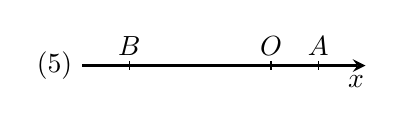
\begin{tikzpicture}[scale=0.6]
		\node[left] at (-1, 0) {(5)}; 		% 左编号
		\draw[->, >=stealth, line width=1pt] (-1,0) -- (5,0); 		% 绘制水平线
		\node[below] at (4.8,0) {$x$}; 
		\foreach \pos/\label in {0/B, 3/O, 4/A} {
			\draw (\pos, 0.1) -- (\pos, -0.1);
			\node[above] at (\pos, 0) {$\label$};
		}
	\end{tikzpicture}
	
	% 图(6)
	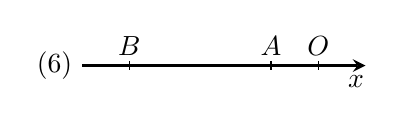
\begin{tikzpicture}[scale=0.6]
		\node[left] at (-1, 0) {(6)}; 		% 左编号
		\draw[->, >=stealth, line width=1pt] (-1,0) -- (5,0); 		% 绘制水平线
		\node[below] at (4.8,0) {$x$}; 
		\foreach \pos/\label in {0/B, 3/A, 4/O} {
			\draw (\pos, 0.1) -- (\pos, -0.1);
			\node[above] at (\pos, 0) {$\label$};
		}
	\end{tikzpicture}
	
\end{document}
